\section*{Zadanie 35.}
\begin{task}
	Wyjaśnić do czego wykorzystuje się rozwiązanie równania Laplace`a w teorii linii TEM. Naszkicować pola
	\textsl{E} i \textsl{H} w przekroju najczęsciej stosowanej linii z klasy "quasi-TEM". Wyjaśnić jakie cechy
	i parametry odróżniają ją od tych linii, które dokładnie spelniają założenia klasy TEM.\\
\end{task}

\begin{solution}
	Prowadzona fala TEM - zmienność poprzeczna
	\begin{itemize}
	\item pola są potencjalne (bezwirowe) w płaszczyźnie XY
	\item mogą być opisane jako:$\\\vec{E_{\perp}} = -\nabla_{\perp}U$\ (*)\\
		$\nabla_{\perp}\vec{D}=0$\     $\nabla_{\perp}\vec{E_{\perp}}=0$\\
		co\ prowadzi\ do\ równania\ Laplace`a:\\
		$\nabla_{\perp}^2U=0$    (*1)
	\end{itemize}
	Funkcja otrzymana z równania (*1) pozwala na określenie ${\vec{E_{\perp}}}$ z równania (*)\\
	Z własności rozwiązań równania Laplace`a:
	\begin{itemize}
	\item fale TEM nie mogą się rozchodzić w liniach jednoprzewodowych (z zasady supremum)
	\item rozwiązania z określonymi warunkami brzegowymi są jednoznaczne
	\item zasada superpozycji w liniach wieloprzewodowych\\			
	\end{itemize}
	Metody rozwiązywania równań Laplace`a:
	\begin{itemize}
	\item bezpośrednie całkowanie
	\item rozdzielanie zmiennych
	\item odwzorowanie konforemne
	\item metoda Monte-Carlo	
	\end{itemize}

	Niesymetryczna linia paskowa (linie mikropaskowe (quasi-TEM)\\
	\textbf{przekrój poprzeczny:}\\
	\begin{center}
    $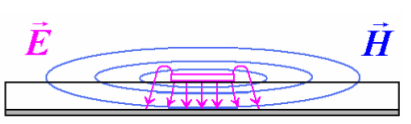
\includegraphics[scale=0.7]{35_1}$\\
    \end{center}
	\textbf{przekrój wzdłużny:}\\
	\begin{center}
    $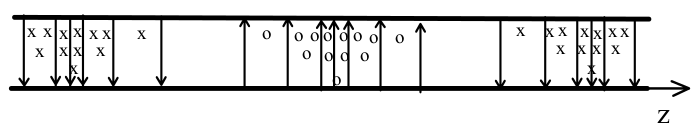
\includegraphics[scale=0.7]{35_2}$\\
    \end{center}
	Cechy niesymetrycznej linii paskowej:
	\begin{itemize}
	\item zależność dlugości fali od szerokości linii
	\item zależność parametrów od częstotliwości (dyspersja)
	\item gorsze odseparowanie od pól zewnętrznych oraz promieniowanie	
	\end{itemize}
\end{solution}